\documentclass[12pt]{article}
\usepackage{times}
\usepackage{fullpage}
\usepackage{fancyhdr}
\usepackage[pdftex]{graphicx}
\usepackage{algorithm}
\usepackage{algpseudocode}
\usepackage{qtree}
\usepackage{titlesec}
\usepackage{textcase}
\usepackage{abstract}
\usepackage[bf,center]{caption}
\usepackage{subfigure}
\usepackage{mathtools}
\graphicspath{{./}{figs/}}
\setlength{\headheight}{15.2pt}
\setlength{\voffset}{-20pt}
\setlength{\topmargin}{-35pt}
\setlength{\headsep}{40pt}
\setlength\absleftindent{0.5in}
\setlength\absrightindent{0.5in}
\setlength{\footskip}{80pt}
\newcommand{\mytitle}{Artificial Life Creation Comparing Genetic Algorithms and Genetic Programming}

\renewcommand{\thispagestyle}[1]{} % do nothing

\pagestyle{fancy}
\fancyfoot{}
\fancyhead{}
\renewcommand{\headrulewidth}{0pt} % remove lines as well
\renewcommand{\footrulewidth}{0pt}
\fancyhead[R]{\small \it{Tom Cammann}}
\fancyhead[L]{\small \it \mytitle}
\fancyfoot[R]{\small Page \thepage}
\fancyfoot[L]{\small \it 183 CS/2012/UG/TC/1}

\captionsetup[figure]{labelformat=simple, labelsep=period}
\titleformat{\section}
	{\normalfont\large\bfseries}{\thesection.}{1em}{}
\titleformat{\subsection}
	{\normalfont\normalsize\it}{\thesubsection.}{1em}{}
%\titleformat{\subsubsection}
%	{\normalfont\normalsize\it}{\thesubsubsection}{1em}{}

\begin{document}
\title{\LARGE \bf Artificial Life Creation Comparing Genetic Algorithms and Genetic Programming\vspace{1cm}}
\author{\small Tom Cammann\\
\small \it{School of Systems Engineering, The University of Reading, UK}}
\date{}
\maketitle

\renewcommand{\abstractname}{}
\begin{onecolabstract}
\noindent \it Abstract - This report focuses on generating artificial life through two distinct methods, genetic algorithms and genetic programming. The
report describes the fundamentals of these two methodologies, compares and contrasts their differences in the creation of similar 
artificial life. The report outlines tools developed during this project to accomplish an effective comparison of these two methods.
These include a method of visualising the artificial life and the environment it inhabits during its existence. The outcome of 
this project demonstrates how genetic programming requires more advanced programming but can lead to novel and emergent behaviour,
in contrast to genetic algorithms which are much simpler and can better replicate biological processes that go on around us. 
\end{onecolabstract}


\section{Introduction}

Artificial life or Alife is the study and implementation of systems that are simulations or replications of natural life~\cite{adami98}.
These systems can be biochemical, mechanical, computer software, or any other medium that supports the existence of structured self controlled information.
This report will be looking at software artificial life, or Soft Alife and how it can be implemented using evolutionary computation.
Evolutionary computation has been used for the creation of artificial life for many decades with the field of study first beginning in 1986~\cite{mit99}.
Koza demonstrated the use of genetic programming to  in 1992 to solve the ant's nest problem~\cite[~p.329]{koza92}. This used a set genes as available
commands for the simulated ants to use, such as move forward, turn, move to nest. The ants problem was an ordering problem on a set of resources on a simple
2D map. This simple example showed how Alife could be used in the context of genetic programming.
Using evolutionary computation has many qualities that replicate naturally evolved life, and is one few computational methods known that
can generate computational solutions to problems without human interaction~\cite{koza91}.
Evolutionary computation has been applied to artificial life to generate life forms that can inhabit an environment and are 'solutions' to this environment.

\paragraph{}
This project also aims to develop an application that can be modified and extended; providing relevant documentation, adopting established design
patterns and developing readable source code. This application will facilitate the running of two evolutionary computation algorithms and will allow
custom goals to be set for these algorithms. Different environment and challenges can be developed for the artificial life to solve using the 
genetic algorithms, with easy-to-use structured code set up to allow the extension and alteration of these environments for new and further
usage of the application. This application will also provide real-time feedback to the user about the algorithms progress and the life forms
this algorithm produces. This will allow quicker understanding of whether the right implementation has been chosen and provide great visual feedback
to confirm the correct implementation has been chosen. The application will also allow in-depth simulation of the Alife, with the ability to 
run the Alife on a previously saved environment or a new randomly generated one. The simulations can be paused and slowed, and run through 
step-by-step, to help better understand the Alife generated.


\paragraph{}
Evolutionary computation generally works by generating a population of solutions to a problem, and then using this population to create a better generation that can solve the given problem better.
To create a better population crossover, mutation and selection are used in various forms to generate a fitter population.
Each of these populations is referred to as a generation.
Each member in the population is a solution to the problem, however these solutions do not have to be correct, and are often close to correct before many generations have passed.
Each member of the population is assigned a fitness value to correspond with how close the solution is to correct, or how effective the solution is.
In the context of artificial life this fitness value may correspond to how well the life form survives in a given environment.

\paragraph{}
The purpose of this investigation is to compare and contrast the usage of genetic algorithms and genetic programming in the creation of artificial life.
Genetic programming (GP) first became prevalent in the early 1990 after Koza used GP to solve many real world problems such as the creation of an antenna
which performed better than previous man-made designs~\cite{koza05}. After the advancements made by Koza, many
applications for GP emerged and one of the earlier applications was in Alife. Before these advancements genetic algorithms (GA) were the primary method for generating Alife.
However these two algorithms have very different implementations and usage, this report will investigate the usage of both in the context of artificial life creation. 
Being able to compare this two types of algorithms will enable faster and better selection of algorithms during 
the design of an artificially evolved life form. It can be a very daunting prospect to choose an algorithm
for developing and evolving artificial life; there are many factors that will need to be considered and this
project will help future research into artificial life by comparing the two algorithms used in this project.
Both these algorithms will have their benefits and pitfalls; exposing these in this report will enable better understanding of which algorithm to choose.


\paragraph{}
This project will design and implement an application which will launch and visualise the evolution of a
simple artificial life form. This application will make use of either genetic algorithms or genetic programming,
depending on conditions chosen at run time, this application will then generate an artificial life form that will navigate a given environment.
The initial parameters for the creation of Alife can be chosen before run time. During run time statistics of the evolutionary process will be produced, and
graphing the fitness over generations will show how the evolutionary algorithm is doing. There will also be an interface to visualise the life  algorithms form in its
environment. This will give the use the advantage of being able to study the behaviour of the life form and understand its behaviour better
than reading the genome.

\paragraph{}
Research on choosing an algorithm for artificial life is fairly sparse and almost none on a direct comparison between the two algorithms. There are also
very few research articles on the generation of artificial life using JGAP or creating a framework for evolution that can accommodate multiple 
evolutionary algorithms. The research done in this project shows novel use of software to compare two evolutionary algorithms in the pursuit of
artificial life.

\subsection{Requirements}
Comparing evolutionary algorithms in a fair and equal way has certain challenges. First, both of the algorithms have to be implemented in such a way that allows a direct comparison. 
This can be done by constructing an environmental problem for artificial life to solve, and then implemented either evolutionary algorithm to solve the problem. Direct
comparisons can be made on how these algorithms were implemented and how efficient and effective they are at solving the given environmental problem. This
environmental challenge can then be changed, and the algorithms reimplemented and a comparison can be made on how well the algorithms can be adapted to the new
problem and again how effective the algorithms were at finding a solution to this problem.

To setup these environmental problems for the artificial life to solve, an environment needs to be constructed in which either of the algorithms can generate
an artificial life form to inhabit.

\paragraph{}
This interoperability between the two algorithms will also carry over to the visualisation of the artificial life. This will mean
that the visualisation and statistics generated about these artificial life forms will have to be abstract and produce similar results regardless of
whether the Alife was generated through a GA or a GP, this information will be encapsulated. This will increase the ease of which the algorithm output can
be compared. However this will pose a challenge to program; to be able to implement the same functionality between the 
different algorithms. For example if the life form has a sight function or 'ability' this need to be programmed for both
the GA and GP because of the way the two algorithms work. These need to give the same response in the same situation. One of the
algorithms can not have advantages over another.
	

\section{Analysis}

\subsection{Key Problems}
Producing artificial life that can solve the environmental and situational problems that are presented in the simulated environment 
was the biggest problem to overcome in this project. Generating artificial life is a complex process; first an environment to simulate the artificial life has to be produced, and then
an interface between the artificial life and the environment has to be implemented. Finally the process for creating artificial life through a GA or GP can be produced, but these algorithms
both need to interface with the artificial life in an abstract manner so one can not distinguish between an GP implementation of artificial life and a GA implementation.

\paragraph{}
The first problem identified was producing an environment for the artificial life. This environment will support the artificial life and allow interaction between the resources present
in the environment and also other life in the environment. The environment that the artificial life will inhabit will be fairly simple with several parameters than can be affected such as
size, and objects for the artificial life to interact with. These objects that the artificial life can interact with will either be resources which the artificial life can possible consume
or an obstacle which the artificial life cannot move over, instead bypass. Keeping this environment simple will enable this project to focus more on producing a high quality artificial life
which will interact correctly and effectively with their environment. 

\paragraph{}
Another problem identified is what methods and values would be used when comparing these two algorithms. To draw conclusions from this project the data generated from both algorithms needs 
to be comparable but also similar. Simple methods for comparing the algorithms will be runtime, memory/space requirements to compute a solution to a give problem. Further detail will need to
be drawn from the algorithms, such as average fitness of a whole generation of artificial life forms, the effectiveness of the algorithm to find a global optimum solution and also the
intelligence of the artificial life produced. 

Producing these statistics will require the algorithms to be generating information that can be interpreted by a statistical model to be translated to graphs and values that can be
used to directly compare the algorithms. This will be done by implementing a several class that will aid this process, objects that can read in an entire generation of life forms
and record information about these life forms. 


The key issues with this project are based around a fair comparison of the algorithms. 

\section{Genetic Algorithms}

Genetic algorithms were first became a main stream theory in the 1970s when John Holland published his ideas on the future of evolutionary 
computation. His book 'Adapation in Nature and Artificial System' in 1975 laid the ground works for modern genetic algorithms. However due to computation
power of the computers at these times genetic algorithms did not take off until the 1980s when the average desktops computational power became
high enough to allow any practical application of genetic algorithms.

The general form of a genetic algorithm uses genes to represent parameters inside a program.
These parameters effect the running of a program.
These genes were historically represented in binary form, however more modern implementations can use any value as a gene, from programming objects to double floating point numbers.
These genes must be able to mutate, this is easy to understand when using binary number, to mutate a binary number you flip one bit in the gene sequence. 

\begin{algorithm}
\caption{Pseduocode for a simple genetic algorithm}
\label{fig:garun}
\begin{algorithmic}
%\Function{GenerateInitialPopulation}{$popsize$}
%	\State $population \gets ( )$
%	\For{$i = 0 \to popsize$}
%		\State $i \gets i + 1$ 
%	\State $population + randomGenes$		
%	\EndFor
%	\State \Return $population$
%\EndFunction

\State $pop = GenerateInitialPopulation(100)$
\State $pop \gets assignFitnessToEachMember(pop)$
\While{$time > allowTime$}
	\State $newPop \gets selectMembersOfPopForCrossover(pop)$
	\State $newPop \gets mutatePopulation(newPop)$
	\State $pop \gets assignFitnessToEachMember(pop)$
	\If{$highestFitnessInPopulation(pop) > fitnessRequired$}
		\State \Return $fittestMemeberOfPopulation(pop)$
	\EndIf
\EndWhile
\State \Return $fittestMemeberOfPopulation(pop)$


%\State $population =$ GenerateInitialPopulation()
%\State evaluate( $population )
%\Repeat
%\State $pop \gets 10$
%\State select fit individuals for crossover and/or elitism
%\State generate new individuals through crossover and mutation
%\State replace old generation with new individuals
%\State evaluate fitness of each individual in population
%\Until { fitest individual \geq fitness required OR time elapsed \geq time allowed } 
\end{algorithmic}
\end{algorithm}

\subsection{Population Representation}
In genetic algorithms each member of the population (or candidate solution) is represented by a list or string of values.
Each value represents a parameter that will be used in the solution.
The value could represent the number of iterations of a loop or represent a operator in a sum.
Traditionally binary numbers strings were used to represent a member of the population.
This was because of the ease of which this could be manipulated by computers and the simplicity mutations could be achieved.
To mutate a binary string a bit can be flipped.
This can work in most situations however it soon becomes apparent that this cannot useful in all situations.
%Fix and show formula? Find solution.
If numbers are being represented in binary strings the most significant bit is at start of the string, if this is flipped 
then the number will change by a factor of ???.


\subsection{Mutation}
In genetic algorithms mutation occurs on a per gene basis. In the configuration of the genetic algorithm there will be a value which 
determines the likelihood of a mutation on a gene within an individual. This mutation is usually applied after or during crossover ~\cite{goldberg1989genetic}.
This mutation can vary depending on the precise implementation. The mutation can cause a complete gene change, meaning the gene before mutation will
have no impact on the new gene, you can also have a variance mutation in which the mutation will cause a change in the current gene. A variance
mutation on a integer gene would change the value represented by this gene by a set amount in relation to the original value. The mutation could be \(\pm5\)
which would cause an integer gene of 81 to change to a maximum of 86 or a minimum of 76. This project actually makes use of the variance mutation, as it is 
better for narrowing in on a local optimum, and most of the simulations used in this project the local optimum is usually the global one.

\section{Genetic Programming}
%intro to gp
Genetic programming is one of the newest forms of evolutionary computing. 
%different ways
The run of a genetic programming algorithm is very similar to that of the genetic algorithm given in figure ~\ref{fig:garun}. An initial
population is constructed and then the fitness is computed. Individuals are selected for crossover and mutation which then forms a new 
population to repeat this process on. The main difference between genetic algorithms and genetic programming is in genetic programming
the program to evaluate is the individual in contrast to genetic algorithms where the genes represented in the individual are applied to
a program for evaluation~\cite{whitley94,gpintro98}. Each individual in the population represents an entire program, rather than a set of values which can be
applied to a program. 

\subsection{Population Representation}

In genetic programming there is a variety of ways to represent a solution. Genetic algorithms are most
commonly represented in tree form which was first made popular by Nicheal Lynn Cramer after publishing his research in 1985~\cite{cramer1985,conf1985}.
Other methods of representing a genetically programmed solution such as a graph pose a greater programming/implementation 
challenge~\cite{gpintro98, poli99}. These more complex method were out of the scope of this research project and so a easier
to implement tree based system has been used.
The software package used to build the genetic program had very good support for tree based genetic programming which made implementation
of this project much quicker, this was another reason the tree based representation has been chosen.
Using this method or representation, the solution to a given problem is made up of node genes, each gene represents a function or variable
which the life form can execute or reference.
This tree will contain only one root node and this node will be executed first, subsequent nodes can have a varying arity. The choice of
which node will be executed next will depend on the function node that was last executed. If the root node had an arity of two, then
the next node to execute will depend on the outcome of the root node. Figure ~\ref{fig:tree1} shows a simple program represented in
tree form. This is the standard form that a genetic program will take. Any non leaf node is a function and the leaf nodes are terminals.
Functions can be any type of function that takes in at least one input (an arity of at least 1) and returns a value. A terminal is a
function that does not take any input or a variable. In figure ~\ref{fig:tree1} the leaf nodes are the numbers 4, 19, 8 and 12 in this
case. The functions are addition (+), subtraction (-) and multiplication (*). These functions all have an arity of two and therefore
require two input, or two sub nodes. Evaluating this example tree gives:

\begin{math}
( ( 4 + 19 ) + (12 - (8 * 4) ) )
\end{math}

%TREE
\begin{figure} [ht]
%\centering
\Tree [.+ [ [ {4} {19} ].+ ] [ 12 [ 8 4 ].* ].- ]
\caption{Genetic Programming tree solution \label{fig:tree1}}
\end{figure}


To expand on this example we can replace the basic math functions of addition, subtraction, etc with functions that the Alife can
do or carry out that require input and receive and we can replace the terminal with either state variables or with functions that do not 
require an input. These functions could be checking for a wall ahead or checking for life, could issue a command to turn a certain
amount or any other command that the Alife is programmed to carry out that requires an input. The terminals could also be functions
such as move forward, which do not require any input or can be simple state variables such as y position or x position on a given map.
The program trees can be also made more complex by adding control statements into the tree. Figure ~\ref{fig:tree-if} shows a visual
representation of this. The IF node requires 3 child nodes; the right most child is evaluated first, this the control statement. If
the control statement is evaluated to a value above 0 then this gives a true response. If a true response is received from this 
child node then only the second child node is evaluated (the middle node). If the control child node evaluates to false, only the 
left most node is evaluated. As we can see from figure ~\ref{fig:tree-if} the LifeAhead terminal will not get evaluated, as the 
control statement child \(5*0\) will evaluate to 0 which is considered false, and therefore only the true branch will be evaluated.

%TREE
\begin{figure} [ht]
%\centering
\Tree [.+ [ [ 5 0 ].* {LifeAhead} {WallAhead} ].{IF} [ {SmellFood} {LifeBehind} ].- ]
\caption{Control statement tree \label{fig:tree-if}}
\end{figure}

\subsection{Mutation}
%asdsss

Mutation of the genetic program is handled by JGAP, however when and how much this mutation occurs can be altered through JGAP
configuration. The genetic code of each life form is made of of nodes on a tree, each of these nodes can be mutated by either
replacing the node or removing the node. The nodes can be replaced with an another node with the same arity and type, the
removal of node is fairly simple can is done by replacing the node with a null node. This will be a empty child node and
will just end execution if this node is reached during the trees execution.

\subsection{Crossover}

As specified earlier this implementation is using trees, this means that the crossover during the evolutionary computation
will work through the tree representation. Using trees for representing your solution means that genetic cross over is
very simple. Two solution trees will first be selected for crossover, this selection will be based around the fitness of the given
solutions. This selection could be done several through several methods and is left to be explained elsewhere. Once two trees
have been selected for crossover and that the return types of all the nodes is the same, then the process of crossing over
is fairly straight forward.

Figures ~\ref{fig:treesab} and ~\ref{fig:resultanttrees} demonstrates a crossover at node C on tree ~\ref{fig:tree-b} and 4 on tree ~\ref{fig:tree-a}. In
figure  ~\ref{fig:treesab}, giving the two resultant trees in figure ~\ref{fig:resultanttrees}.

\begin{figure} [ht]
\centering
\subfigure[]{\label{fig:tree-b}\Tree [.A [ D E ].B [ F G H I ].C ]}
\hfil
\subfigure[]{\label{fig:tree-a}\Tree [.1 [ 4 5 6 7 ].2 [ 8 9 ].3 ]}
\caption{Trees to be crossed over.\label{fig:treesab}}
\end{figure}

\begin{figure} [ht]
\centering
\subfigure[]{\label{fig:tree-Ra}\Tree [.A [ D E ].B 4 ]}
\hfil
\subfigure[]{\label{fig:tree-Rb}\Tree [.1 [ [ F G H I ].C 5 6 7 ].2 [ 8 9 ].3 ]}
\caption{Resultant trees after crossover, around node C and 4 \label{fig:resultanttrees}}
\end{figure}


\section{Development}

This project was written in Java programming language and was developed on several operating systems during its life time. 
Java was chosen because of a strong prior intimate knowledge of the language and because of the libraries available to develop with. 
The evolutionary computation libraries which this project are based also use Java, this made interfacing with them very easy. 
Another reason Java was chosen was because of the graphical user interface programming libraries supplied as standard in Java. 
Having prior knowledge of these also meant that developing a visual format for the simulation could be accomplished.  Along with using 
Java for development several other tools were used these were Eclipse, Maven and Git. Eclipse is a integrated development environment or 
IDE which provides the user with an interface with faster programming and debugging abilities than are available as standard.
This meant faster development. Maven was used a build tool to manage dependencies and build jar files for running the application 
that contains the simulations. Using this made it easy to develop on any computer, as managing the dependencies necessary for the 
program done all by Maven. Git was used as the version control system for this project, this was only adopted towards the 
end of the project as it became more necessary to manage versions and have a reliable branching system. This project was hosted 
on GitHub.com which meant that development could quickly begin from any location with git available. 

\subsection{Design and Architecture}

Before implementation the architecture and design of this project was laid out in UML. The actual design has changed somewhat since the first UML diagram was
constructed, however this was expected and planned for. Figure ~\ref{fig:umldiag1} shows the first UML design for this project.
Most software projects usually have changing requirements and aims during their life cycles as did this project. The project 
used a software development cycle akin to agile software development, where first a feature list was made up with consolation, this
list contained all requirements for the upcoming sprint in the project. These features were then implemented in the project, such
as developing new features in the user interface. These features were then rigorously tested and fixed where necessary. Then 
the cycle was repeated again, drawing up a new feature list.  This project consisted 3 sprint periods where new features 
were drawn up, implemented, tested and bugs fixed.

As Java was the language being developed the design was very focused towards object orientation; this meant using the concepts 
of encapsulation, abstraction and polymorphism. The map design revolved around encapsulating all life, resources and obstacles 
under one object, making this overall object only expose necessary attributes and readonly methods. This meant the underlying 
objects would not be disturbed by any GUI or user interface functions that exist on top.  

\begin{figure} [ht]
\centering
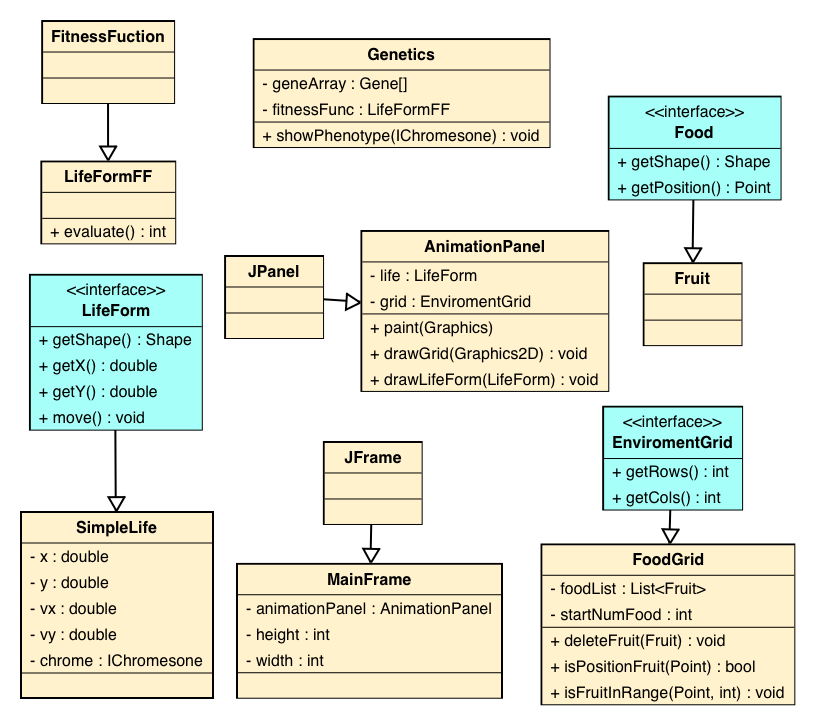
\includegraphics[scale = 0.5]{uml1.png}
\caption{First UML Project Design}
\label{fig:umldiag1}
\end{figure}

\subsection{Project Design}
The requirements of this project were to create a evolutionary computation implementation along with a application to visualise and
display the Alife created by the evolutionary computation. Breaking down the requirements we can see there are two many aspects
the evolutionary computation and the visualisation components, these two components are fairly abstract and do not need to alter
each others states during execution the application. The visualisation only references the Alife and does not need to alter
the Alife, and the Alife does not need to know of the existence of the visualisation; the same goes for the evolutionary framework
in which it does not need to know the existence of the visualisation and the visualisation does not need to alter any state or
information this program may contain. Visualising the Alife presents a common programming problem, in which we have a model a view and a controlling
device. The view will be the graphical user interface, which will display the animation of the Alife inside its environment, the 
model will be the environment in which the Alife inhabits and the controller will be the Alife. This problem has a generic programming
solution or architectural pattern called Model View Controller (MVC)~\cite{fowler03}. This pattern facilitates separation or responsibility
and independence between these three components. The application designed followed this model, figure ~\ref{fig:mvc} demonstrates 
how this model can be applied to this application. The arrows on this figure demonstrate which components interaction, a leading arrow
shows that this component interacts and may alter the component it is point to.

\begin{figure} [ht]
\centering
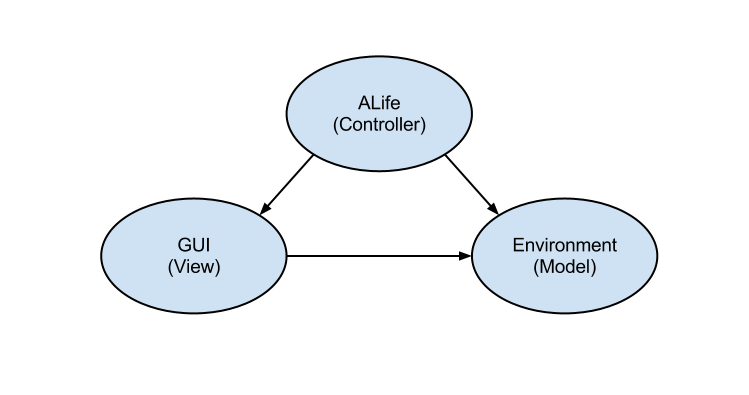
\includegraphics[scale = 0.5]{mvc.png}
\caption{Model View Controller architecture for project application}
\label{fig:mvc}
\end{figure}

The application developed for this project created several high level interfaces to allow for this model, and the development for each
component was done separately. Development of one component, eg. Alife controller would not affect any development of the visual 
GUI components.

\paragraph{}


\begin{figure} [ht]
\centering
\subfigure[Genetic Algorithm Alife architecture]{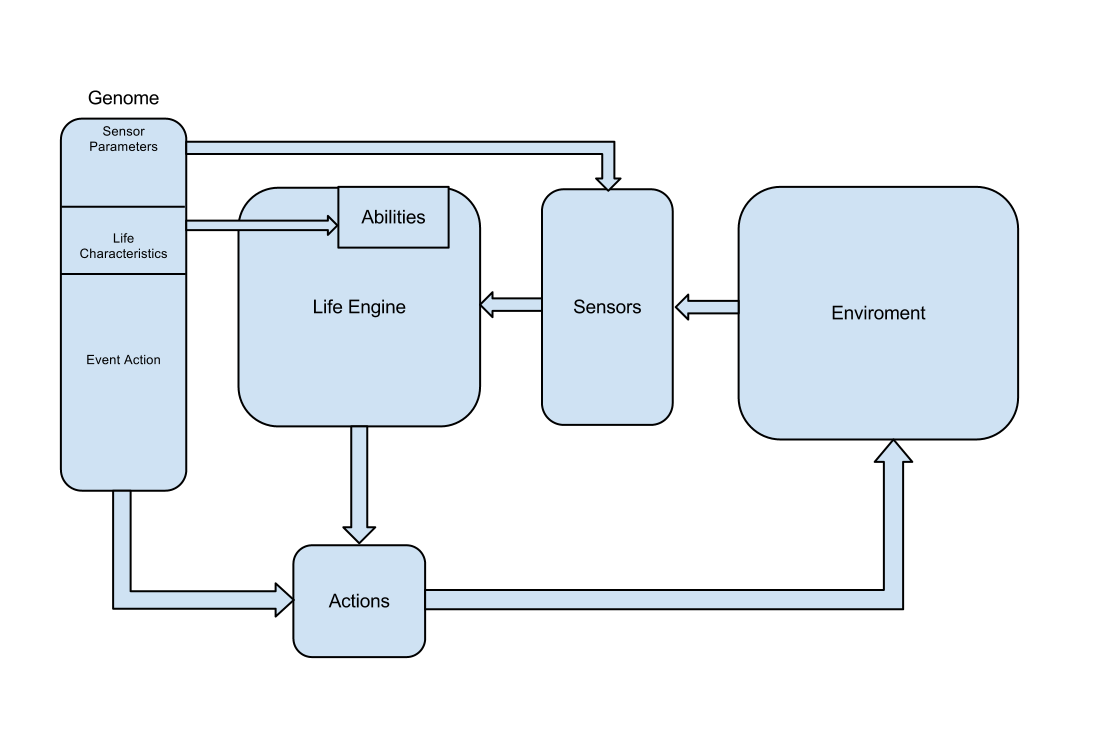
\includegraphics[scale = 0.3]{alife-arch.png}}
\subfigure[Genetic Programming Alife architecture]{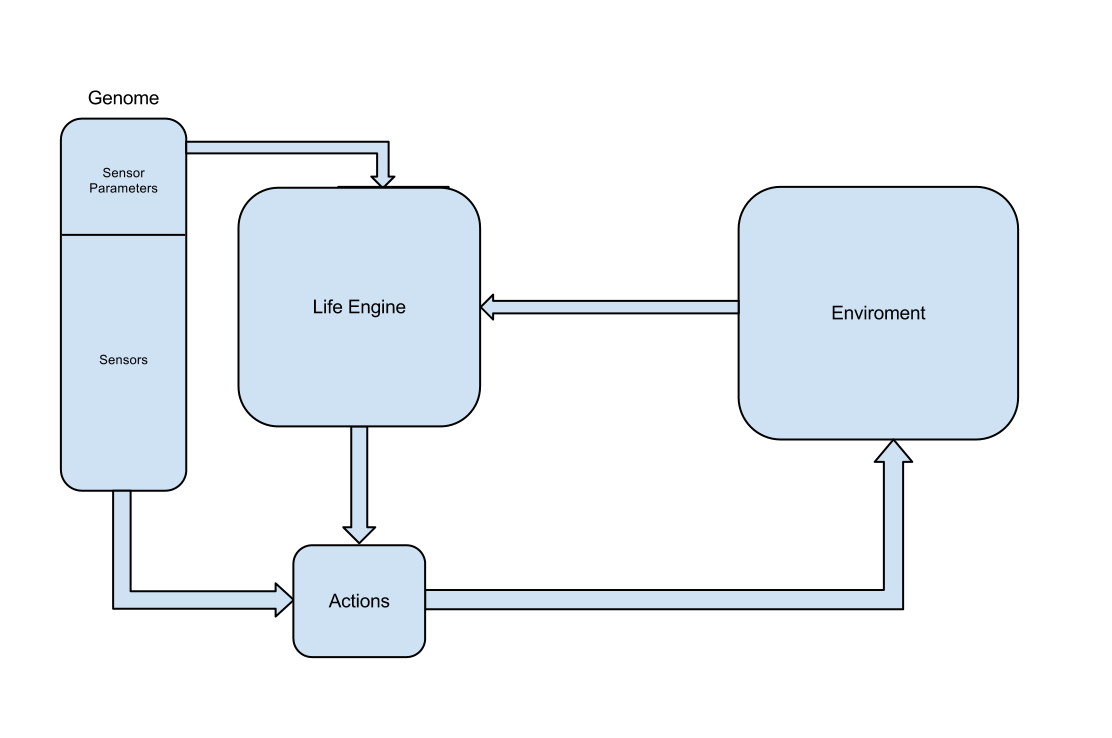
\includegraphics[scale = 0.3]{gpalife.png}}
\caption{Architecture design of the artificial life between the two algorithms}
\label{fig:mvc}
\end{figure}


\section{Implementation}
To evaluate a common artificial life form a simulation environment has been created.
This environment is a 2D arena where a life form must continue to consume food to survive, the more food the life form consumes the fitter the  

The underlying genetic and evolutionary computations were completed on a Java framework called JGAP (Java Genetic Algorithms Package).
This package provides a tried and very well tested method for using genetic algorithms in Java, while also providing the 
ability to extend the package and use the package to fit into this projects needs. The package was tested several times before usage
and simple life forms were developed to ensure this package was appropriate. Other packages such as %TODO other packages
were used but found to be lacking extendibility and documentation. JGAP has very good documentation, which meant that extending
the package and adapting the package to this projects needs was even easier.

JGAP provides two general over arching algorithm frameworks to work with, genetic algorithms and genetic programming. However
the package does not provide any high level interfaces between the genetic algorithms side and the genetic programming side. A 
lot of development during this project was focused on developing a framework for evolution that could incorporate both GAs and GPs developed
using JGAP. 

Visualising both the GP and GA in the life form meant developing an abstract way of representing the state of the life form. This was done
through an abstract class called Alife. This abstract class provided a high level interface for other objects to read (and modify if necessary)
the state of the life form. The abstract class contained many of the variables for the life form and the setting and getting functions 
associated with them. 

\subsection{Life}

This project has modeled life on upon a fairly simple scenario, with only a few state variables. The states that this life form
can control are: its position on the map, its orientation and its energy level. Its position can be changed by moving forward, these 
forms can only move in the direction they are facing. The can modify their orientation by moving either right or left of where they 
are currently facing. They can also change their energy, however this is more passive than active. The life form's energy will
deplete during its life based on how much it moves and what actions it takes. However its energy can be increased by consuming a 
resource, this resource will contain a number of calories which can be converted into energy. This conversion rate is variable
depending on the life forms parameters. 

The simulation is split up into frames, during each frame the life form has a chance to move and interact with the environment. If their
are multiple life forms in the environment then each life form in turn will get a chance to interact during this frame. These frames are
meant to represent time for the life forms, it has been slightly simplified to be an amount of time a life form can move forward or interact in another way. Only one 'major' interaction can be completed per frame. These include moving, consuming a resource and turning.

To survive in an environment the life form must keep its energy above zero for the duration of the simulation, if the life forms energy
drops to zero or below then the life form will be assumed deceased and can no longer make any more interactions with its environment. A simulation can have indefinite run time and how long the life form can survive will depend on its fitness and availability of resources for energy.

When a life form needs to be tested for fitness it is added to a map, and the life form is asked to make an action for every frame. The life form starts out
with a nominal energy value, so that it does not die at the start of the simulation. A fit life form will then make intelligent actions and move towards resources
that it can consume to increase its energy level. The fitness of the life forms is accessed usually assessed by its energy level at the end of the simulation. 


\subsection{Map}

The environment that the life forms exist on during the simulations are referred to as maps. These maps are two dimensional and can vary in size.
The size of the map can be set at run time and can also be set to dynamically change during a run if necessary. The map also holds references
to the resources contained in the environment. The map is split up into cells which form a 2D grid for which the life forms can inhabit. 

Generally for evolving good fit life forms a unique map is generated for each simulation. This creates an environment in the life form has not
seen before and has not adapted to before. This means that the fit life forms are the ones which will be able to adapt to any give situation
and still be able to consume and interact with their environment. Each time a map is generated a new set of resources is generated with different
positions on the map and different calorie values. If a static map is used, with the same positions of resources for each run, a very specialised 
life form can evolve but as soon as this life form is transposed into another environment this life form is very unfit.

The resources generated for each map are randomly placed, with random calorific values. Only one resource can occupy a cell on the map, each resource also has
a type which can be checked by the life form. If a life form is on top of a resource, i.e. if it is in the same cell then the life form can consume a resource. 
 

\subsection{Evolutionary Framework}
To investigate and compare these two algorithms a framework to accommodate both algorithms was designed and implemented. This framework had to allow comparison
of the effectiveness and fitness of the life forms evolved, efficiency of the 
evolutionary computations in generating a fit life form and the correctness of the solutions generated. To enable all these things an abstract framework had 
to be developed to allow comparison without respect to the algorithm that was used. This first accomplished by visualising members of the population and 
manually inspecting the fittest life form of each generation. 


\subsection{Visualisation}
Visualisation of the solutions (or life forms) produced by the algorithms was key
to understanding the differences produced in the life forms between the two algorithms. A visualisation of the map and life form
was developed early on. The visualisation was developed using the model view controller architecture,
which meant that the map and the life form were completely detached from the visualisation.
The life form was made abstract by using an abstract class which contains the basic variables need for the life
form and some simple functions to get and set these variables. These include the life forms position, orientation
and energy level. The visualisation renders the 2D map with resources on, with the cell size depending on the attributes selected at runtime. The frame speed can
adjusted during the visualisation, but is default set to 5 frames per second. The visualisation itself is contained within the visualisation window. This window
provides access to the visualisation such as start, stopping and restarting the simulation.

The visualisation has also been used to debug the life forms produced, to find errors in the project code which the life forms have ended up exploiting. An example
of this was during early development their existed a bug that cause the life form to stop decrementing its energy when it got to a map corner. When the simulation
was run with this bug in the life forms would evolve to find the corners of the map as they could get stuck their and never die. These life forms were not that fit 
as they usually only had a fitness value that was around their starting energy.

Later in development other features were added to the visualisation window. One of these features was the ability to import and export maps for the life forms to be
tested out on. A previously generated made could be loaded and the life form could be assessed on how it dealt with the that particular map. Producing this ability meant that it would be easier to compare life forms, understanding exactly how they interacted with the same environment.
Another feature that was added was the ability to run the simulation frame by frame. The user can pause the simulation and step through the simulation, this again provides another method of fully understanding how a life form interacts with the environment. 
Along with the abilities to interact with the simulation was the ability to access information on the current life form, such as its genetic make what generation
and run time parameters were involved with its creation.

\paragraph{}
Along with being able to visualise the artificial life form in an environment, there is also the ability to visualise the
evolutionary process. A high level view of the processes occurring underneath is available during a standard launch of the
main application. First is a graph displaying the fitness across the evolutionary generations. This graph shows in real-time the
average, maximum and minimum fitness of all the artificial life in each generation.

This can however be a significi

\subsection{PROGRAM FLOW}

\section{Problems Encountered}

During implementation many hurdles had to be overcome during each sprint phase of the project. However there were some issues that were much harder to overcome than others. One of these problems was
producing fair and equal output per time frame from each algorithm. The problem was that during each time frame the artificial life had the opportunity to survey its environment and then react to this
environment, hopefully in a way such that it can find more resources to consume, but the rules governing these interactions differed between the two algorithms.
This was because of the way the two algorithms generate output which controls the life form it was difficult to align
the rules governing the two algorithms. Originally the genetic programming solution controlled the artificial life by calling functions with in its chromosome tree, such as move forward, turn left etc.
However it was quickly realised that this would not work as the genetic program could call these functions multiple times during one time frame. This method would not work in this project because
of the way the genetic algorithm controls the artificial life. The GA did not have an opportunity to call functions multiple times during one time frame. These methods of control had to be aligned. 

This was a difficult problem to solve, either the genetic algorithm had to modified in such a way that meant it could call interaction methods
a number of times or limit the number of calls the GP could make to these interactions. It was deemed easier to modify the GP, and a solution
was devised to fix this issue. The solution was to change the way the GP controlled the Alife. Instead of directly calling the interaction methods
the GP would instead return a number, this number would then refer to a specific action. The interactions that could take place in 
the environment are then hard coded into the program, e.g. if 1 is returned the Alife turns left, if 2 is returned the Alife turns right.

\paragraph{}
Another problem encountered was during refactoring of the code. Towards the end of the project the code base was fairly substantial, and any
untested modification to the code could produce errors. During some refactoring of the EnvironmentMap class several bugs slipped through
which meant a longer than necessary amount of time was spent debugging. However due to this project adopting the software version control system
Git, a 'diff' or file comparison could be made on the changed files. For the refactoring a new branch was created on git, the refactored code
was then developed on this refactoring branch, and the working code remained on the master branch. When the bugs occurred in the
projects code the file comparison between these two branches was extremely helpful in locating exactly what had been changed and what
possible bugs could have arisen from these changes. In this particular case a method that was acting as the sight for the artificial life
contained an erroneous 'not' symbol causing havoc. Initially it was hard to understand where the bug had arisen as many methods had been
altered, but using git diff, a tool for comparing files, meant I could easily inspect the changes and quickly went through any changes would could have produced the
results that were being produced by the project.

\section{Results}

Results obtained from the project showed expected but interested outcomes. The results cover the whole Alife creation process including
development and implementation of the evolutionary computation. The results showed how much effort and technical skill was needed to
implement each of the algorithms and how effective and responsive the Alife was to its environment.

\subsection{Effort in Implementation}

After the general framework for the evolutionary computation was developed the genetic algorithm was implemented. The JGAP package used
was straight forward to use and after some time reading documentation and other resources about JGAP it was simple to implement a basic
Alife program. However this program did not receive any output from the environment, these elements could not be directly programmed into
the genetic algorithm. The main bulk of implementation and testing was done on the Alife sensors. These sensor could not self evolve or 
create themselves as there is no mechanism for complex recombination of variables in genetic algorithms. Once the sensors were developed
the parameters for these sensors could be fed in from the genetic algorithm. The genetic algorithm then optimises the sensors to suit
the environment best. The other genes that were programmed into the Alife for the genetic algorithm were other Alife characteristics
such as memory length and variables that effected some life abilities. These variables were also optimised during the run. Introducing
these variables into the genome was straight forward, and expanding on the current genome to add more genes would be a trivial process.
The genetic algorithm produced good results during development too, as more sensors and more genes were added to the Alife the results
improved and showed a strong correlation between more sensors and higher fitness. This meant that development could be incremental allowing
instant testing. The actual runtime of the GA was quicker than anticipated, this enabled the project to increase the population size which
was initial meant to remain around 1000 to around 2000.

\paragraph{}
The genetic program took much longer to develop and refine. The was less documentation and resources available for genetic programming 
development in JGAP but that will not be taken into account. The complexity came in developing genes for each of the sensors. Each sensor
needed to be encapsulated inside a gene, which either required an input and produced output or just produced output. The output between
the genes had to also be standardised to a certain type to allow interoperability between the genes. The genes produced in this application
all produced primitive doubles, which caused some issue with some of the sensors. As the program structure was made up during runtime by
the genetic program, the genes had to be completely abstract. The run time for these programs was actually faster than that of the GA due
to the fact many of the solutions generated were much smaller than the GA Alife produced. This meant that the average run time was much 
less overall. However this was not always the case as some run configurations created GP solution trees that were much larger than the 
GA solutions, these took much longer to evaluate and caused a slow down for the entire genetic program. The implementation of the GP was 
more of a technical challenge as well, requiring a greater understanding of Java and of evolutionary computation. Understanding and debugging
was a longer and more drawn out process, as the Alife program to be debugged was hidden behind the GP tree inside the JGAP interface.
This would hold true for any other implementation of a GP, the code being run inside the evolutionary computations is hidden away. If strange
structures arise inside the tree such as a loop in the tree it can be very hard to detect as the only real output is the log and
the tree structure. Once the genetic program was stable, the process to extend the Alife's capabilities and sensors was a simple one. Before
runtime genes can be enabled and disabled for usage during the evolutionary computation. This means that genes can be hotswapped between
runs and results can be directly compared to understand the impact that change had on the run. An example of this was disabling the turn
right gene in one particular run. The fitness took more generations to climb to the fitness achieved by the run with both turn right and
turn left. This shows how much more resilient the genetic algorithm is to change in the genome, it is able to adapt better to changed in
the environment also.

\subsection{User Interface}
To help in the comparison of the two algorithms a user interface was developed. There are several cal parts to the user interface, the main
interface was the Alife visualisation. This interface has been robust and very informative throughout the project, providing valuable
feedback about the Alife the from both algorithms. Figure ~\ref{fig:interface1} shows this main interface, using a small sized map.

\begin{figure} [ht]
\centering
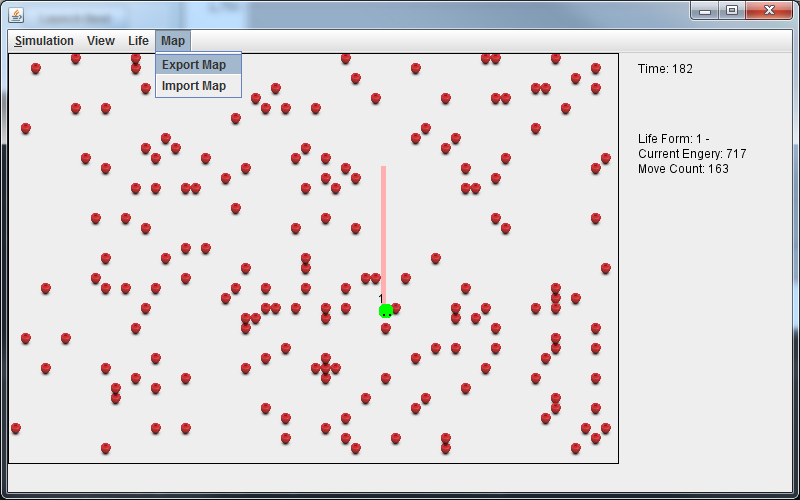
\includegraphics[scale = 0.45]{smallvis.png}
\caption{GUI for visualising Alife}
\label{fig:interface1}
\end{figure}

This figure shows the interface rendering a small map, with resources placed upon the map, these are the red apples. The interface can
render multiple life forms on the map at one time, and render different types of resources that the life form may consume. The animation
or image for each object on the screen is handled by the Java object represented by it. This means that the animation for the green
Alife form in the center is controlled by the Alife. The color of the Alife, or size, or shape could be manipulated by the evolutionary
computation also. Along with the Alife visualisation, there is a real-time graph showing the fitness  across the generations of the 
evolutionary computation. This graph is updated as the evolutionary computation moves through generations. This can be seen in figure
~\ref{fig:nicegraph}. This figure has the highest, lowest and average fitness achieved for each generation across 60 generations. This
graph is also easily extensible allowing more data to be visualised with the minimum of effort thanks to the framework developed in
this project.

\begin{figure} [ht]
\centering
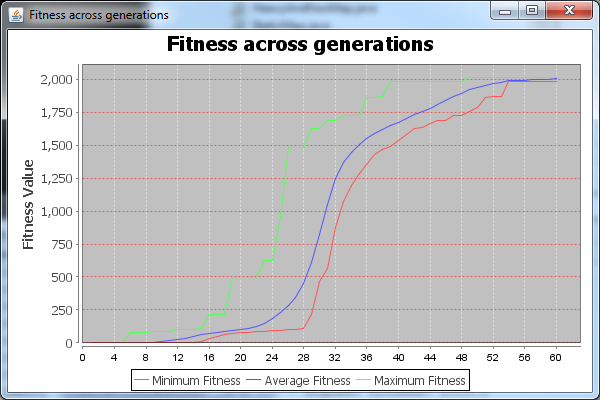
\includegraphics[scale = 0.6]{nicegraph.png}
\caption{real-time graph showing fitness across each generation of the evolutionary algorithm.}
\label{fig:nicegraph}
\end{figure}
%Environment change

\begin{figure} [ht]
\centering
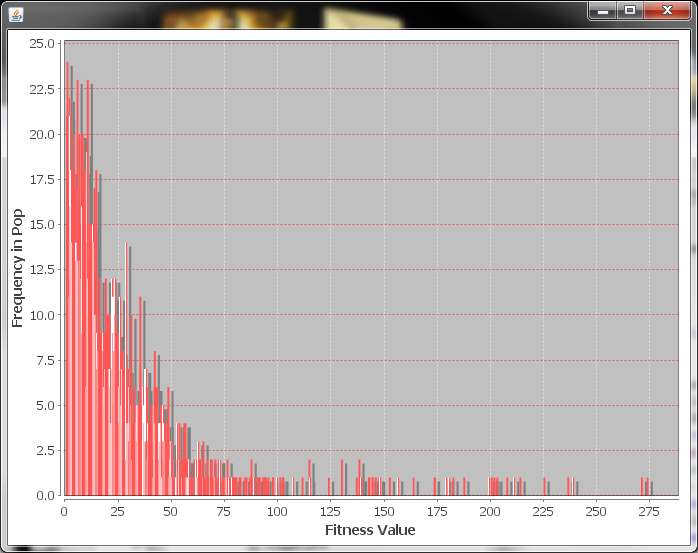
\includegraphics[scale = 0.75]{gen0-2500.png}
\caption{Fitness distribution of one generation from a genetic algorithm run.}
\label{fig:graph2500}
\end{figure}


\begin{figure} [ht]
\centering
\subfigure[Generation 1]{\label{fig:gen0graph}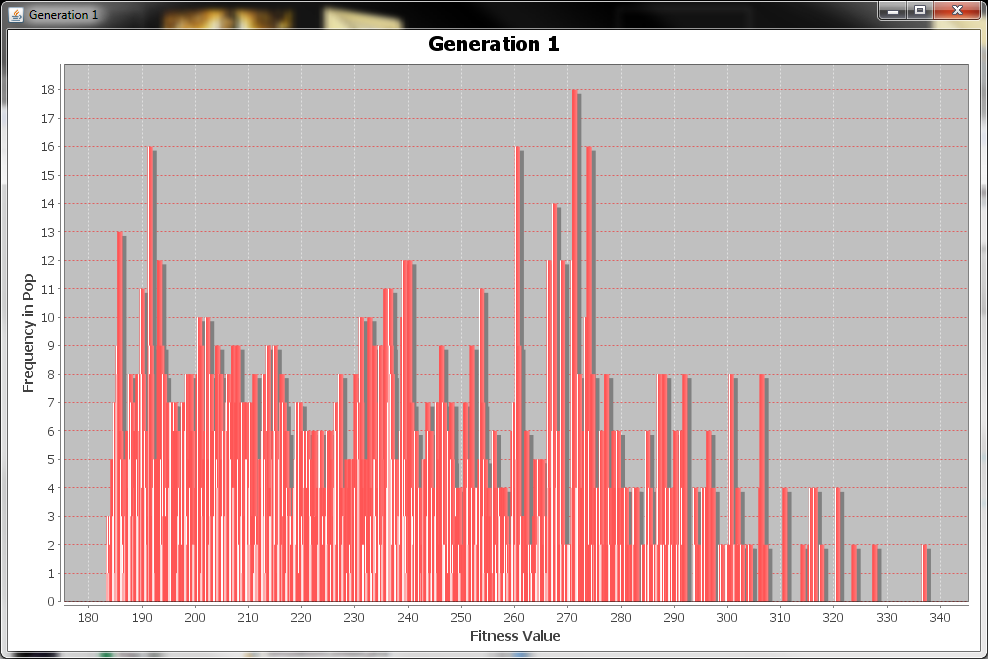
\includegraphics[width=60mm,height=30mm]{gen.png}}
\subfigure[Generation 2]{\label{fig:gen1graph}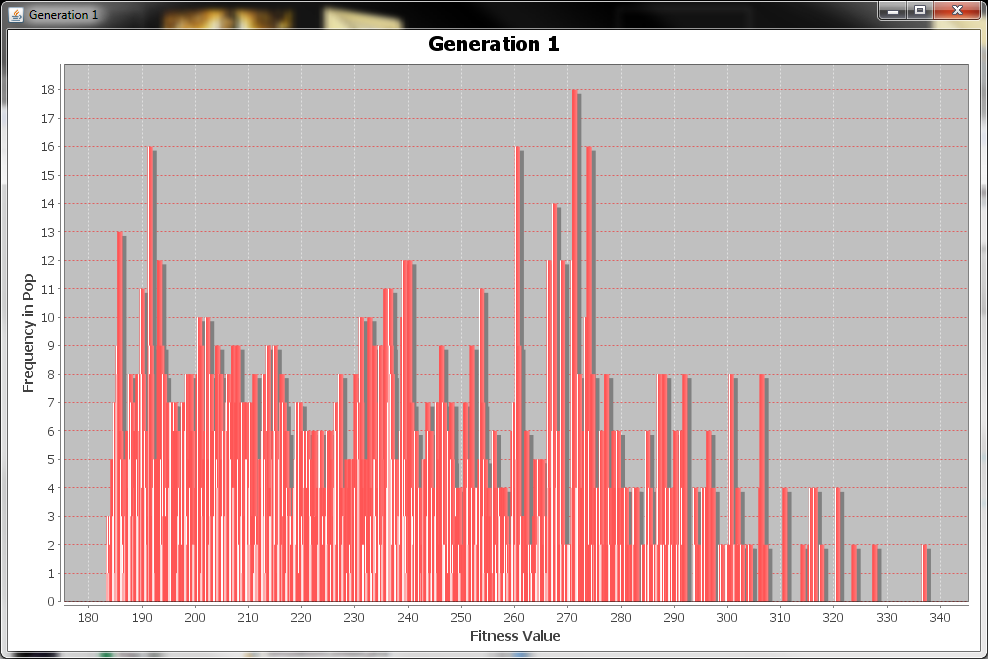
\includegraphics[width=60mm,height=30mm]{gen1-2500.png}}
\subfigure[Generation 3]{\label{fig:gen2graph}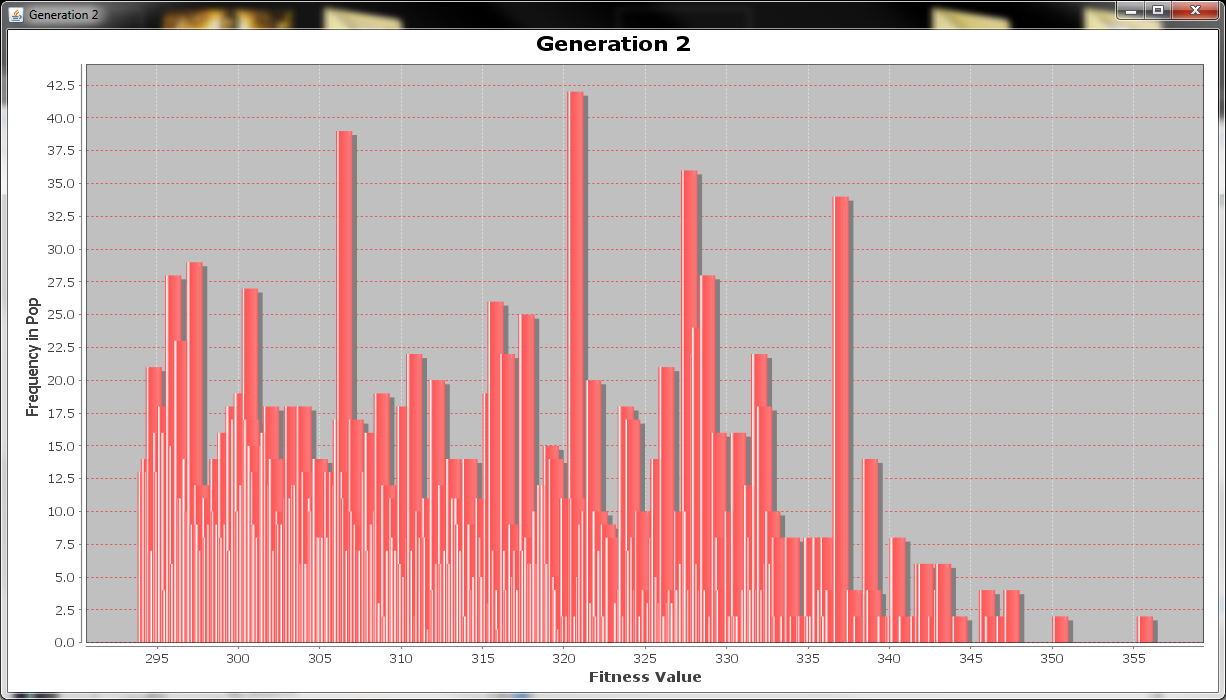
\includegraphics[width=60mm,height=30mm]{gen2-2500.png}}
\subfigure[Generation 4]{\label{fig:gen3graph}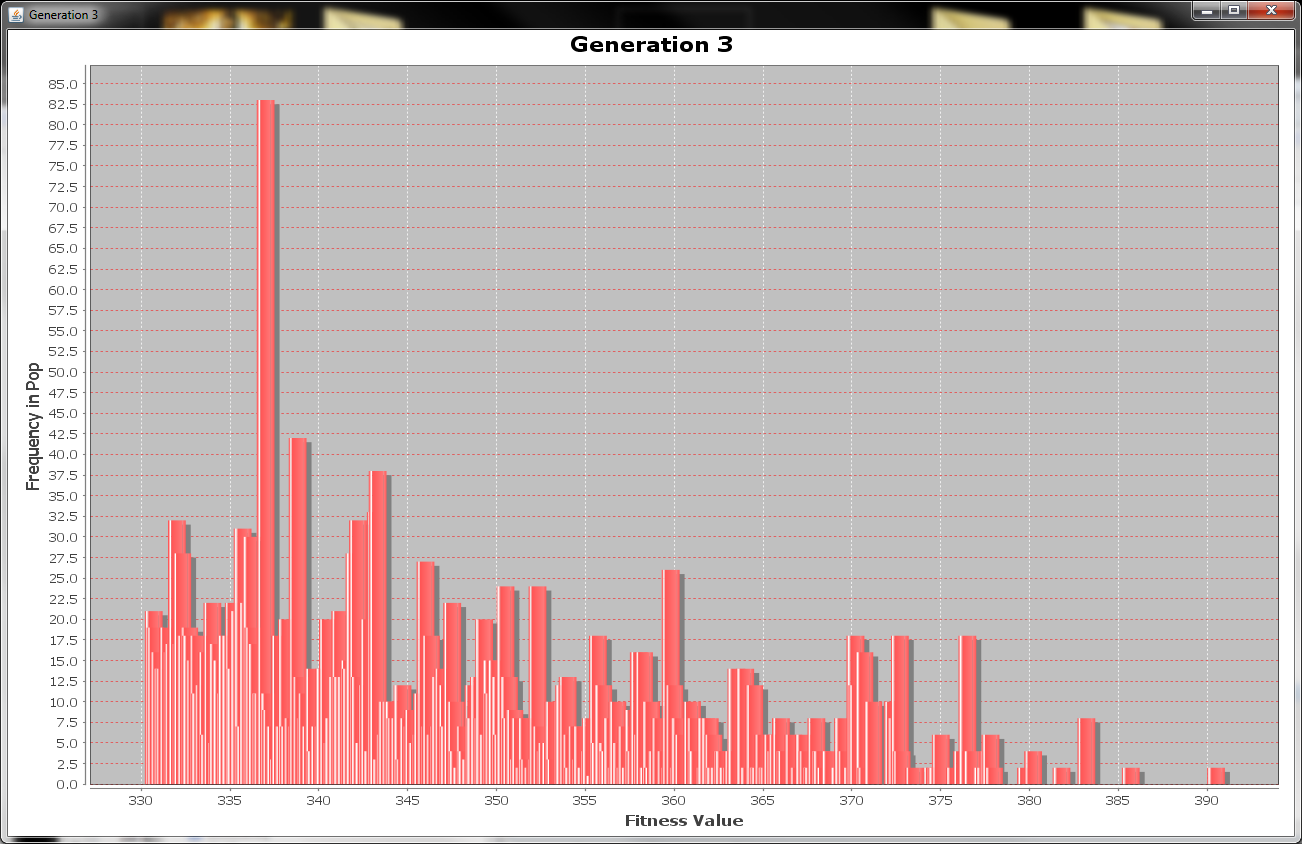
\includegraphics[width=60mm,height=30mm]{gen3-2500.png}}
\subfigure[Generation 5]{\label{fig:gen4graph}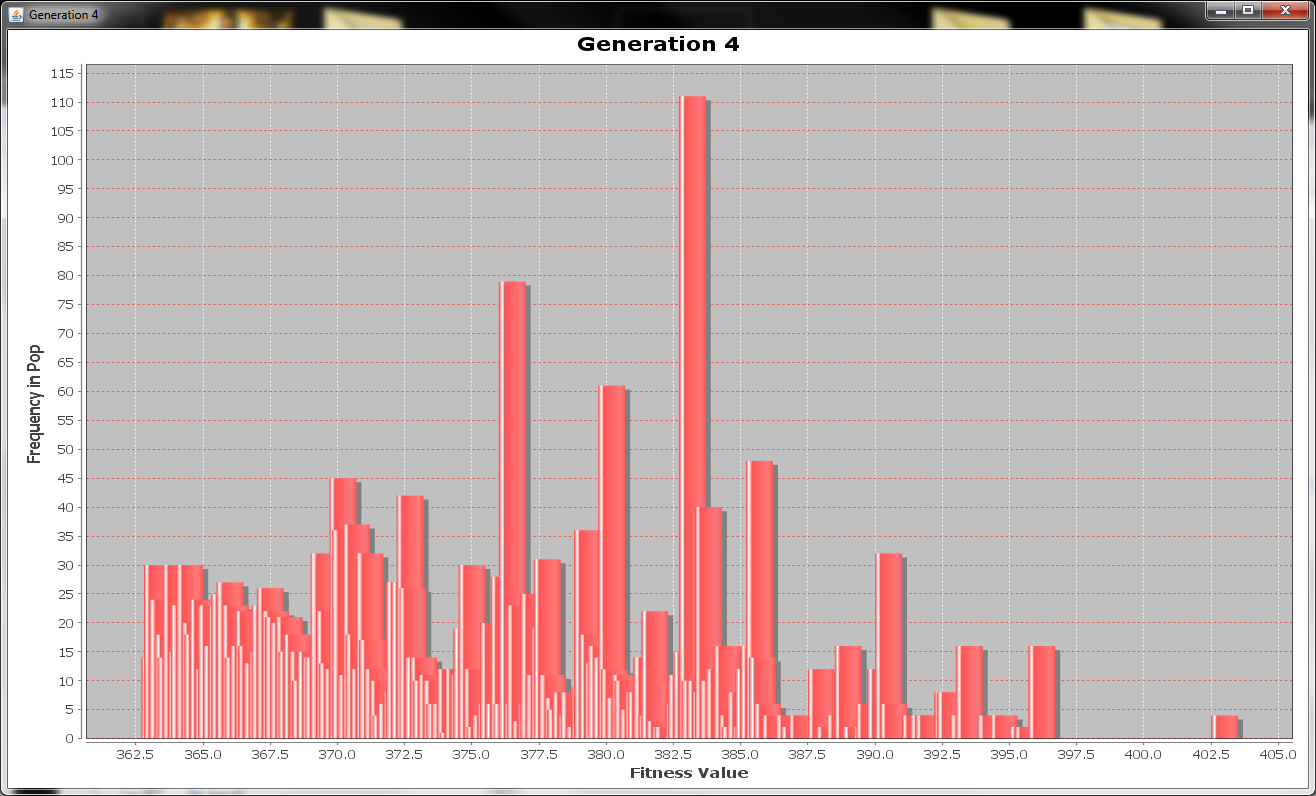
\includegraphics[width=60mm,height=30mm]{gen4-2500.png}}
\subfigure[Generation 6]{\label{fig:gen5graph}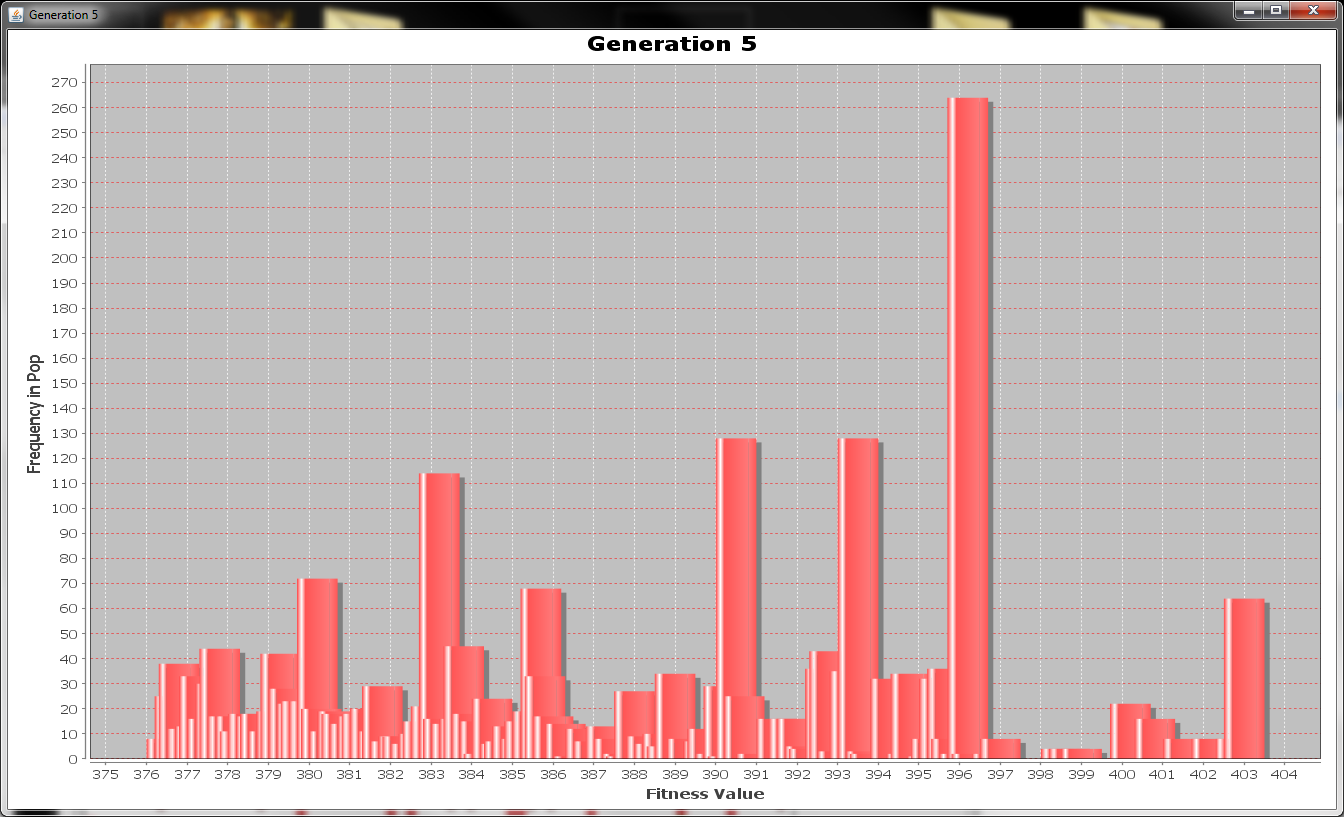
\includegraphics[width=60mm,height=30mm]{gen5-2500.png}}
\caption{Series of graphs show population distribution across 6 generations}
\label{fig:genseries}
\end{figure}

Figure ~\ref{fig:graph2500} shows the fitness distribution a generation of 2500 GA solutions. 

\subsection{Alife Creation}

Creation of Alife through the genetic algorithm and the genetic program was very successful. Both algorithms could solve and complete all of the test
environments that were tested. These environments included, environments with an abundance of resources, environments with sparse resources and 
environments with obstacles. The genetic algorithm was very good at generating a general solution for all situations, and produced fit life forms
very quickly. A run of a map of size 600 by 400 in which there was 150 resources saw a very quick convergence on the global optimum. Within 
15 generations the highest fitness was in 90% of final highest fitness. This life form has 29 genes, with 19 possible actions genes to call.
Using the same environment the genetic program run took fewer generations, only 10 generations, to converge on a fitness within 90% of the global optimum fitness, however
the simulation took 140 seconds longer to compute. The genetic program had 16 possible genes available. 

Simulations with obstacles was the next challenge for the Alife. The genetic algorithm was not as competent at navigating the obstacles as the
program flow was static and could not dynamically adapt to different situations posed by the obstacles. However the genetic program dealt with
the obstacles much better. Convergence on a global optimum took 25 generations with the genetic program with the genetic algorithm not quite obtaining
a fitness as high as the genetic algorithm, converging on a local optimum in 18 generations. The genetic algorithm was still quicker, reaching the 18th generation
in 112 seconds and the genetic program took 279 seconds to reach the 25th generation.


%CREATION OF ALIFE.
%implementation
%evaluation
%adaptation - how well the Alife adapted.
%extension, different environments. 


%Ease of extension to other Alife

\section{Discussion}

The main point to draw out of the results is the success of creating artificial life from both genetic algorithms. Along with this point the 
visualisation of artificial life was also successful, a high quality GUI was produced that enabled viewing and interaction with the Alife.
The code produced for this project has also been of very high quality. The main aim of this project however was the comparison of artificial 
life generated by two distinct evolutionary algorithms and this has also been successful. The aims outlined in this project have been fulfilled.

\subsection{Comparison of Artificial Life}
The results obtained were what was expected, both algorithms produced artificial life that converged upon the global optimum within 30 generations
for all environments tested. The artificial life showed that more complex problems could be solved, this was demonstrated by the navigation around
obstacles in the environment which was handled well by both algorithms however the genetic program managed to solve the problem of navigation much
more succesfully than the genetic algorithm. This was because the dynamic way in which the the genetic program can execute its commands, the genetic
algorithm has a static implementation of its program flow. This is a major limitation for genetic algorithms. To adapt the genetic algorithm to the
new environment with obstacles would have meant redesigning the underlying program with in the Alife and not just modify the genes. This is a major 
consideration when developing artificial life, if your environment is chaning it will be much more costly to develop a genetic algorithm due to the 
fact that the underlying logic will need refactoring if the environment is modified beyond what the Alife is programmed to solve. The genetic 
program was very good at dealing with this new scenario, however its run time was longer than that of the genetic algorithm for both situations. The 
run time has been discussed previously in this report and is longer than that of the genetic algorithm because of the dynamic way in which solutions
are formed, creating some very long programs. 

These results show that if time and computational power are not of issue then the genetic algorithm creates more adaptable and 


\section{Testing}
The main goal behind testing this project was to ensure complete correctness of the implementation which utilises the JGAP framework.

Unit testing was one of the main tools used for this project. JUnit 4 was used in this project and was chosen for this project because
of its high renown in software engineering, and is usually the de facto standard choice for any testing in Java. It provides a robust framework
in which tests can be written and run with ease. JUnit also integrates extremely well with Eclipse, the main IDE used during this project. Eclipse has default plugins for running and writing JUnit tests making the whole testing process even easier. Any test
failures will be shown, along with an exact reference on screen to where they failed. Individual test methods can then be run and
debugged to enable the code being test to be fixed very quickly.
This project also utilised Maven 3, Maven has the ability to run JUnit tests and generate reports from these tests. Using the Maven
Surefire plugin and enabling reporting from these tests produced very useful reports on the project in HTML, although these were not
that useful as most of the tests were run through Eclipse. However Maven really comes into its own when other testing plugins are
utilised. This project used the Maven Cobertura plugin, Cobertura is a ''tool that calculates the percentage of code accessed by 
tests'' - http://cobertura.sourceforge.net. Using the Cobertura with Maven's reporting capabilities meant that detailed reports
on exactly what code was being tested by the unit tests. The HTML reports produced show the exact source code that is run during the
testing. This meant that JUnit tests could also be checked for correctness, and that any code that needed to be tested has not been
missed out.
Another tool used for testing was FindBugs, this tool used static code analysis to find errors in Java source code. This tool also
has a Maven reporting plugin which produced more HTML reports in readable and easily accessible format. FindBugs assisted in finding bugs in the projects code which would have otherwise been missed. FindBugs not only finds bugs and issues with the logic in the code
but also assess the performance, security, style and code convention. Many trivial issues can be raised by FindBugs such as 
incorrectly defining static fields or other simple programming mistakes. It can produce very useful feedback for producing
higher quality code and helps the programmer avoid common mistakes and improve efficiency of the code. The find bugs report breaks
down the issues it finds by class, and then by priority. Most reports generated during this project contained many 'low' priority
issues such as: ''uses the same code for two switch clauses'', these issues are often ignored due to the fact they are artifacts
from code that is still in development, but occasionally a 'high' priority issue arises and these that often need to be immediately
addressed in the code. 

This project also used
CheckStyle for helping the code adhere to strict Java programming code conventions. Adhering to these code conventions meant that
the code produced is more readable, easier to understand, easier to debug and helps avoid bugs.

This complete strategy for testing was chosen as it enabled this project to focus on development of the code and spend as little
time as possible on developing tests. This streamlined testing process improved the efficiency of the project, tests could 
be written, tested and verified in very little time. Using Cobertura the tests could be verified that they were covering the
correct areas, FindBugs, CheckStyle improved the readability and transparency of the code and also helped stop static code
bugs occur.


\paragraph{}

The Unit tests written for this project were aimed at the most important and complex areas of code. Exhaustive testing was 
unfortunately of the scope of this project, and full test coverage of the entire code was not feasible to implement.

This project focused on implementing test driven development, TDD, which meant writing unit tests alongside writing project code.
This increased the work load but was essential to ensure correctness of the code being produced. Major benefits were seen from
writing these unit tests concurrently with the project code. Bugs that would have very hard to track down from a mis-assigned
variable were very easy to locate. Performance of the code was also improved, due the fact that each time JUnit runs the test
it also reports how long this took. Using this it was easy to see which parts of the code are very inefficient and which needed
refactoring. 

However the 
areas of the code that could produce 'silent' bugs were targeted for testing. A silent bug is one which would not throw an error
or even produce erroneous output, but would perhaps alter the outcome of a run slightly. A example of this was a method that
was used as the eyes of the Alife in the genetic algorithm. The range value is taken from the set of genes, and is used to 
to limit how far the artificial life can see. The method that was written accidentally reduced this range by 1 due to an issue
in incrementing a for-loop. This bug was not spotted until a test for this method was written. 
\paragraph{}

The logging used in this project was implemented through Log4j, this system enabled this project to customise the logging 
ability without costing the project runtime. During debugging the trace log can be enabled which will slow down the
run time of the project but provide invaluable help when debugging the code. When logging is turned off the performance
of the code has very similar performance to code with any logging statements in, this makes Log4j very powerful. Also
Log4j has many built in output and format options which means one can customise it to suit any project. Log4j is often
thought of as industry de facto logging platform and therefore is highly supported meaning increased performance
and one of the safest logging platforms in terms of the number of bugs because of its age and community support. All these
factors contribute to a highly effective and stable logging platform. 

Log4j has several levels of logging, fatal, error, warn, info, debug, trace. Each of these logging levels can be used throughout
the project, however logging in this project was used with a strict set of rules. Any errors or erroneous outcomes will 
be logged as either fatal or with error level logging, fatal will be used in a case where any further outcome of the project
will be invalid or erroneous, error will be used for logging any error that will cause the current run of the system to be
erroneous however will probably not impact the rest of the run. Warn will be used when parameters exceed recommended
extremes or an acceptable or expected bad input is recorded and adjusted. Info is used for recording the current state of
the project run, for example each time a new generation is started during either the GA or GP run the info logging level is
used to print and record that this is the current state of the program. It is used to record high level state of the run,
not the low level state of each of the components which combine together during this run. Other common info level logging
information would be the fitness of the entire generation or if a target is reached in the code such as a fitness level.
Debug and trace are only used for debugging, and often trace is disabled at run time because of the impact enabling this
logging level has on the code. Most logging that occurs in this project is trace or debug logging, logging statements are
put into frequently used methods and classes to record the current state that they are in and to help during the debugging
process. The trace log level is used for calls that are very frequent and if not disabled would likely produce a significant
low down during runtime. 

\subsection{Test Alife}

Testing the correctness of the Alife was a slightly more complex task, and could not be completely automated through unit testing.
The common errors that occurred during development of the project which affected the Alife simulation were normally due to the
artificial life evolving to exploit bugs in the simulation. One such bug allowed to the artificial life to never die by exploiting
a case were it could skip code that required energy to decremented at the end of each turn, and therefore the Alife did not need
to consume resources to become fit.

Another common bug would be where the Alife would get stuck in the corner of the map and not be able to escape this corner. This
was an error to do with the Alife's navigation and movement commands.

These bugs were discovered by inspection and not through automated testing. This meant these bugs took longer to find and longer to
debug. Automated tests could not be written for the Alife as there was not an expected behaviour to test against. The best
test for these artificial life forms was the fitness function. The life form would be successful and pass the tests if the fitness
was above a certain threshold. Through a particular run of the project if the fitness outcomes were exceptionally high or close to 
zero then this run would probably have a bug in the implementation of the project and would be inspected. When this occurred
it was often a time costly bug as the cause would not be given and would have to be found. However the tools developed in this
project helped greatly in finding these bugs. The first one was using the visualisation frame, an Alife form could be chosen
and run on a chosen map. The artificial life could then be debugged by stepping through its life, using the visualisation tools.
Using the verbose logging setup throughout the project and the ability to run the life form time frame by time frame meant that
some bugs could quickly be found through this process. Different maps could be loaded and the whole process reloaded again for
repetitive testing. 


\subsection{Testing The Environment}


\section{Conclusion}
The project has generated interesting findings along with a useful tool for further information gathering. The finds relate to the implementation of each algorithm
showing the benefits of using GAs or GPs within different situations. The application developed allows the easily fine tune a GA or GP and produce visual results 
from its fittest offspring. This tools has been developed with mindset that other developers may with to adapt or extend this application and has therefore
been produced in a readable and documented way. The application produced has been of high quality, with a test driven development, allowing further tests to be
added easily also. The applications GUI is professional looking, with a clean interface and simple to use, allowing the user to visualise and play with the 
Alife that has been created by the evolutionary computation.

The documentation produced along with the code is also of high quality. The main documentation provided with the source code is the JavaDoc. A JavaDoc has been 
written for almost every method and every class, with useful and often detailed description of the method or class. This documentation allows future developers
of this code to quickly understand the code and be able to extend and improve the current code. This JavaDoc is also improves code during development as it 
provides a constant reference to information about any classes used and how they should be used in the context of this application. 
Along with the JavaDoc, the code has used strict coding standards and has adhered to them very well which has produced very high quality code. High quality code
means that the code is readable, understandable and extensible. The code has been designed with extension in mind, producing interfaces and abstract classes
that facilitate these extensions easily.

\subsection{Future Improvements}
The application developed went through a long design process however this design had to be altered somewhat during the implementation stage, this meant that some
features in the design could not be fully implemented in the desired way. An oversight on how the GP would execute its solution left a design flaw within the program,
such that the frame timing between the GP and GA was not equal. If the project was redesigned then this issue could be remedied by creating a different framework for
handling the idea of time within the simulation. Currently time is handled by the EnvironmentMap.java interface, where the incrementTimeFrame() is called, this then
calls each Alife form on the map and ask to to make a 'move'. Ideally this idea of time could be handled independently by the Alife, without deferring to the map for
a call to move. Perhaps the Alife could have a cycle speed in which it can do one action every cycle, where the cycle time maybe controlled by the evolutionary algorithm
or statically set. 
Another design improvement that could be made is to improve the security and abstractness of the code. Currently many classes that do not need access to the Alife
object have access to the Alife object. It was very difficult separating responsibilities for this class into distinct sets which could then be implemented through
interfaces. The biggest weakness of the Alife class is the Brain.java interface that has to be set during the creation of a concrete class. The brain interface
delegates control of the Alife during run time, and has complete control of the Alife. This Brain object needs to be reimplemented to allow better abstract and allow
easier extension. The Brain interface is slightly confusing as the only method it implements is the think() method. This method is called when the Alife is required to
move. The GP Alife implements this interface with only a few lines with a call to the GP solution which then chooses the action for the Alife to execute, whereas the
GA Alife Brain contains all of the sensors for the Alife, and directly controls the flow of the GA Alife.
There are also many other forms of Alife that could be simulated and tested, some testing was done of interacting and symbiotic Alife, however the implementation of
these Alife has not yet been finished. The testing done showed promising results. Simulations run where Alife could produce resources which other could consume, produced
interesting results where the Alife would learn to follow each other as close as possible and occasionally changing directions. This behaviour was
interesting to observer and further study of interacting Alife would certainly be a path this project would take if more work was to be done.
Another general improvement that could be made is to write more unit tests for the application. Currently the test coverage reported by Cobertura is only 31%. This
value may seem very low, but the tests have been focused on the logic portions of the code and the critical code that would cause major error in the code if there 
were errors. With that said, other areas of the code could certainly produce errors that could effect the running of the application. To remedy this, more tests
should be written to increase code coverage and branch coverage. Test coverage should ideally be around 80%~\cite{massol04}.




\bibliographystyle{plain}
\bibliography{disseration}

\end{document}
